% ---------------------------------------------------------------------------
% Version history (visible on page 1 and in the PDF metadata; one line per
% content revision, newest first).  The version counts content revisions; the
% build time on page 1 is generated at compile time (\buildstamp), so it always
% matches the file it is printed on.
%   v1.8  2026-10-25  build stamp is generated at compile time
%   v1.7  2026-10-25  rebuild, no content change (v1.5's build stamp was
%                     recorded before the clock check; this build carries the
%                     correct one, and it is the newest PDF)
%   v1.6  2026-10-25  exact-cell share under the 6.0 ceiling: 9%, not 13%
%   v1.5  2026-10-25  visible version line (version, build time, first version)
%   v1.4  2026-10-25  follow-up section names both bars (opt-in 6.0, default)
%   v1.3  2026-10-25  improvement avenues and related work extended
%   v1.2  2026-10-25  revision after the independent desk review
%   v1.1  2026-10-24  related work, survey table, alternatives, 8 pages
%   v1.0  2026-10-24  first version (two-column LaTeX)
% ---------------------------------------------------------------------------
\documentclass[10pt,twocolumn]{article}
\usepackage[T1]{fontenc}
% Page geometry: ACM sigplan (10pt conference) --- US Letter, 1in top/bottom,
% 0.75in side margins, 2pc column separation.
\usepackage[letterpaper,top=1in,bottom=1in,margin=0.75in,columnsep=2pc,heightrounded]{geometry}
% Fonts: the ACM template pair --- Linux Libertine (text) and Inconsolata (mono).
\usepackage[tt=false]{libertine}
\usepackage{libertinust1math}
\usepackage[varqu]{zi4}
\usepackage{microtype}
\usepackage{booktabs}
\usepackage{array}
\usepackage{tabularx}
\usepackage{xcolor}
\usepackage{hyperref}
\usepackage{amsmath}
\usepackage{enumitem}
\usepackage{multirow}
\usepackage{titlesec}
\usepackage{caption}
\usepackage{tikz}

% ACM sigplan heading styles: bold \Large sections, bold normal-size subsections,
% ragged-right, tight spacing.
\titleformat{\section}{\Large\bfseries\raggedright}{\thesection}{0.7em}{}
\titleformat{\subsection}{\normalsize\bfseries\raggedright}{\thesubsection}{0.6em}{}
\titleformat{\subsubsection}{\normalsize\bfseries\raggedright}{\thesubsubsection}{0.6em}{}
\titlespacing*{\section}{0pt}{1.2ex plus .2ex minus .2ex}{0.55ex plus .1ex}
\titlespacing*{\subsection}{0pt}{1.0ex plus .2ex minus .2ex}{0.45ex plus .1ex}
\titlespacing*{\subsubsection}{0pt}{0.9ex plus .2ex minus .2ex}{0.4ex plus .1ex}

% ACM caption style: bold label, small text.
\captionsetup{labelfont=bf,font=small,skip=6pt}

% Build stamp: taken from the compile-time clock (the same \year/\month/\day/\time
% pdfTeX writes into the PDF's /CreationDate), so the visible version line cannot
% drift from the file it is printed on.  Zero-padded by hand because the engine's
% numbers are not.
\makeatletter
\newcommand{\twod}[1]{\ifnum\numexpr#1\relax<10 0\fi\number\numexpr#1\relax}
\makeatother
\newcommand{\buildstamp}{\number\year-\twod{\month}-\twod{\day}, \twod{\time/60}:\twod{\time-(\time/60)*60} CET}

% ACM link colors.
\definecolor{ACMPurple}{cmyk}{0.55,1,0,0.15}
\definecolor{ACMDarkBlue}{cmyk}{1,0.58,0,0.21}
\hypersetup{colorlinks,linkcolor=ACMPurple,citecolor=ACMPurple,urlcolor=ACMDarkBlue,
  pdftitle={Hardening the Exact-Cell KV Window for --kv q4lm8v},
  pdfauthor={Matthias Kronenberger},
  pdfsubject={Version 1.8, built \buildstamp; first version 2026-10-24}}

\setlength{\parindent}{10pt}

\begin{document}

% Full-width ACM conference title block, then the two columns start with the abstract.
\twocolumn[{%
  \begin{center}
    {\LARGE\bfseries Hardening the Exact-Cell KV Window for \texttt{-{}-kv q4lm8v}:\\[0.25em] Design, Decisions, and a Measurement-First Validation\par}
    \vspace{1.0em}
    {\large Matthias Kronenberger\par}
    \vspace{0.35em}
    {\small Version 1.8 \,\textperiodcentered\, built \buildstamp\ \,\textperiodcentered\, first version 2026-10-24\par}
  \end{center}
  \vspace{1.0em}
}]

\noindent\textbf{Abstract}\par
\vspace{0.6ex}
\noindent
The exact-cell KV window is an opt-in memory/accuracy point for Strata's 4-bit Lloyd KV cache (\texttt{-{}-kv q4lm8v}). A small resident ring of recent cells and a set of sink cells are kept in fp16 while the rest of the cache remains 4-bit. With $S{=}256$ recent cells, $R{=}64$ sinks and the automatic prompt chunk capped at $B{=}6{,}144$, the production point uses 5.29 bit/cell (1,016\,MiB at 128K) against \texttt{int8}'s 8.25 bit/cell (1,584\,MiB), at equal prefill throughput and decode inside run-to-run spread. This paper describes the design, the correctness hardening (A1--A5), and a measurement-first validation. Quality is scored teacher-forced against an fp16 KV reference on three fixed corpora (2K, 4K, and 128K --- the 128K point on two texts), reporting mean KL, p99 KL, top-1 agreement and perplexity with paired per-segment statistics; the KL is computed over the reference's top-64 tokens, renormalized (Section~6.3). The window removes most of the plain 4-bit base's error on the cwe task: 73\% of its gap to \texttt{int8} at 4K, and across the two 128K texts 34--58\% of the plain base's tail mean KL. At 2K its mean KL is indistinguishable from \texttt{int8}'s (0.00702 vs 0.00503, $t=-1.92$, window ahead in 2 of 8 segments); at 4K \texttt{int8} is significantly better on the mean ($t=-3.55$, 7 of 8 segments) but indistinguishable in the answer region; at 128K \texttt{int8} keeps the better p99, the last 1,024 positions and the whole segment on both texts. The result is a 36\% KV-memory saving with a small, measurable KL cost, not an accuracy win over \texttt{int8}. The \texttt{int8} default path stays byte-identical (dump-logits SHA against the previous release); AMD HIP is measured, and CUDA/SYCL builds plus a full cell-to-row parity test remain review gates.
\par\medskip

\section{Introduction}

At long context the KV cache is a large, fixed cost: at 128K tokens the \texttt{int8} default reserves 1,584\,MiB before any expert weights are loaded. A 4-bit KV cache reduces that, but quantizing every cell uniformly costs accuracy on long documents: earlier 4-bit KV work measured document perplexity about 8\% and 12\% above the \emph{fp16 reference} at 1K and 8K context (about 7\% and 13\% above the \texttt{int8} default; Q2\_0, \texttt{q4\_0})\,\cite{strata-kv4,strata-details}. The exact-cell KV window is an attempt to keep the memory saving while protecting the cells that matter most.

The memory landscape assumed here is not the datacenter one. On Hopper- and Blackwell-class NVIDIA hardware, an FP8 KV cache is the production two-times point: vLLM reports degradation within 1--2 accuracy points on its reasoning-suite benchmark and aggregate recovery on prompts up to a million tokens --- a suite-specific bound whose longest buckets show visible variance, and whose head dimension of 256 is where FP8 prefill still regresses\,\cite{vllm-fp8}. A consumer AMD GPU driven through HIP has no FP8 attention path; on such hardware the block-quantized \texttt{int8} default is the deployed two-times saving, and 4-bit is the frontier. That is the constraint the window addresses.

The idea is simple. The most recent $S$ cells and the first $R$ cells (attention sinks) of each cache-carrying attention layer --- on the measured model, the 12 full-attention QSA layers of 48 (Section~3) --- are kept in fp16 in a resident side pool; older cells stay in the 4-bit Lloyd format. The window thus spends exact bytes where the model is most sensitive and leaves the long tail compressed. It is opt-in (\texttt{-{}-kv q4lm8v} plus \texttt{STRATA\_KV\_WINDOW=1}) and never changes the default \texttt{int8} path.

The implementation was functional in principle, but several integration points could fail silently: the host-side prompt chunking, the interaction with KV streaming, the stability of the window grid across model states, and the meaning of uninitialized ring entries. We treated these as correctness issues, not performance issues, and fixed them behind the same opt-in flag.

This paper positions the window against prior and current KV-cache compression work (Section~2), describes the design and its production point (Section~3), records the alternatives weighed against it and why each was left out (Section~4), documents the hardening decisions and the evidence that the default path is untouched (Section~5), sets out the measurement methodology (Section~6), and reports results at 2K, 4K and 128K with a discussion of where the point fits (Sections~7--8). The emphasis is on the methodology and on what the measurements do and do not show; file-level implementation detail is deliberately kept out.

\section{Related Work}\label{sec:related}

KV-cache compression splits into methods that drop cells, methods that store every cell in fewer bits, and methods that do not read every stored cell. The window is in the second family, with one exact overlay. The paragraphs below keep only the mechanisms that share a part with that design. Every number in them is the cited paper's, on that paper's models. None was re-run here.

\begin{table}[t]
\centering
\footnotesize
\begin{tabular}{@{}lll@{}}
\toprule
\textbf{System} & \textbf{Point} & \textbf{Documented outcome} \\
\midrule
KIVI~\cite{kivi} & 2b + recent fp16 & per-channel K, \\
& & per-token V \\
SKVQ~\cite{skvq} & 2b K / 1.5b V & high-precision \\
& & recent window \\
IntactKV~\cite{intactkv} & fp16 pivots & first tokens exact, \\
& & rest quantized \\
RotateKV~\cite{rotatekv} & 2b + sinks & FWHT, sink-aware \\
KVQuant~\cite{kvquant} & 3b per-channel & $<$0.1 PPL \\
& + pre-RoPE & (Wikitext-2/C4) \\
SAW-INT4~\cite{sawint4} & INT4 + Hadamard & paged serving; \\
& & near-lossless (theirs) \\
QServe~\cite{qserve} & KV4, W4A8KV4 & serving speedup \\
& & on A100 / L40S \\
GEAR~\cite{gear} & 4b + correction & low-rank + sparse \\
KVTuner~\cite{kvtuner} & 3.25--4.0b & layer-wise pairs \\
DuoAttention~\cite{duoattn} & head split & full cache only on \\
& & retrieval heads \\
SnapKV~\cite{snapkv} & eviction & per-head clusters \\
H2O~\cite{h2o} & eviction & heavy hitters \\
PyramidKV~\cite{pyramidkv} & eviction & 12\% matches full \\
& & cache (LongBench) \\
\texttt{llama.cpp}~\cite{llama-cpp} & q8\_0 / q4\_0 & block-quantized \\
\texttt{vLLM}~\cite{vllm-fp8} & FP8 & $\leq$1--2 acc.\ points \\
\bottomrule
\end{tabular}
\caption{Documented operating points from the literature and production
runtimes. All entries are the cited works' own published results on their
own hardware and models; they are not comparable across rows.}
\label{tab:survey}
\end{table}

\paragraph{An exact residual on a low-bit bulk.}
This is the closest family. KIVI keeps a fixed fp16 residual of recent tokens and quantizes the rest at 2 bits, per-channel for K and per-token for V~\cite{kivi}. SKVQ keeps a high-precision sliding window of recent tokens and reports 2-bit keys with 1.5-bit values at small loss on its models, up to a 1M context for a 7B model on an 80\,GB GPU~\cite{skvq}. IntactKV keeps the KV of a few pivot tokens, the ones that collect the attention mass, in fp16 and quantizes the rest~\cite{intactkv}. RotateKV protects attention sinks explicitly, reorders channels, and rotates with a fast Walsh--Hadamard transform before a 2-bit code; on LLaMA-2-13B it reports under 0.3 WikiText-2 perplexity degradation~\cite{rotatekv}. PM-KVQ, aimed at long chain-of-thought, stores the first token at higher precision, keeps a recent window, and lowers the bit width only as the block ages~\cite{pmkvq}. The window shares the recent residual with KIVI and SKVQ and the sink retention with StreamingLLM~\cite{streamingllm}, IntactKV and RotateKV. It does not share their quantizers. The exact cells are an \emph{additional} side pool: the quantized row stays, so a missed exact read falls back to 4 bits instead of a hole. No calibration set is used.

\paragraph{Axis, rotation, and which tensor gets the bits.}
KVQuant quantizes keys per channel, before RoPE, into non-uniform datatypes, and reports sub-0.1 perplexity degradation at 3 bits on WikiText-2 and C4~\cite{kvquant}. QuaRot and SpinQuant rotate weights, activations and the KV cache so that 4-bit inference is less outlier-sensitive; SpinQuant learns the rotation and reports a smaller gap than QuaRot's random one on its LLaMA models~\cite{quarot,spinquant}. SAW-INT4, a 2026 serving design, finds that token-wise INT4 plus a block-diagonal Hadamard recovers nearly all of the accuracy naive INT4 loses, once the method must fit a paged cache and a fused attention kernel; heavier schemes added little once that constraint bound~\cite{sawint4}. Strata's 4-bit base quantizes per cell after an orthonormal Walsh--Hadamard, so it sits in that family. A paired on/off ablation of that rotation, on the 16-level base without the window, was a tie at 2K and 4K~\cite{strata-wp}. That tie is not a statement about the production window, about 128K, or about SAW-INT4's INT4. The production split stores K at 16 Lloyd levels and V at 8 in one 4-bit block. A paired K-versus-V bit contrast on Swift did not support a ``keys want the bits'' story ($t{=}{+}0.05$, McNemar $p{=}1.0$\,\cite{strata-wp}). That story is nevertheless the published direction of a 2025 geometry argument, which reports that key-favored allocations retain more accuracy than uniform ones on its models~\cite{spectralkv}. The two results are not a contradiction until they are run on the same model. KVTuner's layer-wise pairs, reported nearly lossless at 3.25--4.0 bits on its models~\cite{kvtuner}, and the token/bit co-tuning of~\cite{top-k} are different axes. Neither is measured here.

\paragraph{Correcting the residual, and not reading every cell.}
GEAR adds a low-rank plus sparse correction on top of a quantized cache~\cite{gear}. Palu compresses the hidden dimension with a low-rank projection and reports that stacking quantization on that projection costs little extra perplexity on its models~\cite{palu}. ShadowKV keeps a low-rank key cache, offloads values, and reconstructs a sparse set at decode; on an A100 it reports up to $6\times$ batch and $3.04\times$ throughput, including on RULER and needle tests~\cite{shadowkv}. A 2026 adaptation result is the caution those correction papers need: low-rank updates recovered 54\% and 76\% of the held-out perplexity gap of a frozen 4-bit cache on two models, but a 2-bit recovery that restored perplexity restored only 11--12 of 180 retrieval cases~\cite{kvadapt}. Perplexity and retrieval are not the same yardstick. Eviction drops cells: H2O by accumulated attention, SnapKV by per-head clusters, PyramidKV by a larger budget in lower layers, Scissorhands by a persistence hypothesis, ChunkKV by semantic chunks~\cite{h2o,snapkv,pyramidkv,scissorhands,chunkkv}. The window does not. Selection without a drop is the other line, and it is the one this model already uses. Quest loads the top pages for the current query~\cite{quest}. DuoAttention and RazorAttention keep a full cache only on retrieval heads and a short cache on streaming heads~\cite{duoattn,razorattn}. Native Sparse Attention trains a hierarchical compression-plus-selection in place of dense attention~\cite{nsa}. The measured model is not that architecture. It is a hybrid whose indexer selects at most 2,048 cells per query (Section~3). The window changes the precision of selected cells that fall in the sink or recent set. It does not change the selection. That last sentence is a static reading, listed as follow-up.

\paragraph{What production ships.}
Table~\ref{tab:survey} collects operating points. They are not comparable across rows. QServe ships a 4-bit KV cache inside a W4A8KV4 stack and reports serving speedups against TensorRT-LLM on A100 and L40S~\cite{qserve}. \texttt{llama.cpp} ships block-quantized KV (q8\_0, q4\_0) selected per cache~\cite{llama-cpp}. \texttt{vLLM} ships an FP8 KV path whose reported degradation stays within 1--2 accuracy points on its reasoning suite, with the caveats already stated in Section~1~\cite{vllm-fp8}. Strata's corner has none of those kernels: one consumer GPU through HIP, no FP8 attention. The \texttt{int8} default is already the two-times point, and this paper moves toward 4 bits. The fair competitor not measured here is a per-channel-K arm, before the rotation, on this indexer cache. It is follow-up work, not a claim.

Code and documentation for the compared systems are listed with the references. Strata's own measurement provenance is in Section~6.6.

\section{Design of the Exact-Cell Window}

We name the machine (a static reading of the compiled \texttt{geometry.hpp}, not a measurement): the measured model is Qwen3.8-Flash-Next, a hybrid of 48 layers in which every fourth layer (layers 3, 7, \ldots{}, 47) is a full-attention QSA layer with the KV cache this paper quantizes --- 12 such layers; the other 36 carry no cache of this kind. A QSA query does not read the whole cache: its indexer selects at most 2,048 cells (plus block rounding) per query. Of the 256 dimensions in a head, the rotary embedding covers 64; the other 192 are not rotated. The indexer's own keys are a separate fp32 store, because a different selection is a different attention. Both facts are the same static reading. The window changes the \emph{precision} of selected cells that fall in the sink or recent set, not the selection itself --- we found no code that forces sinks or recent cells into the selection, and verifying that is on the follow-up list (Section~10). ``Keeps the cells that matter most'' (Section~1) is therefore a precision statement about selected cells, and the eviction comparison of Section~2 is about storage, not about which cells are attended.

Three sizes need distinct words. A \emph{token position} is one context token in one layer; in the 4-bit base its stored cost is 576\,B per layer (K and V together). A \emph{scalar element} is one K or V number --- 1,024 per token position (2 KV heads $\times$ 256, K and V) --- and the rates of this paper (4.50, 5.29, 8.25 \emph{bit/cell}) are bits per element. In the prose, \emph{cell} means one token position's K/V entry in one cache-carrying layer, and a \emph{row} is that position's storage within the layer's cache. \texttt{int8} names the default's block format: 8-bit content with one fp16 scale per 64 elements, 8.25 effective bit/element.

\begin{figure}[t]
\centering
\resizebox{\columnwidth}{!}{%
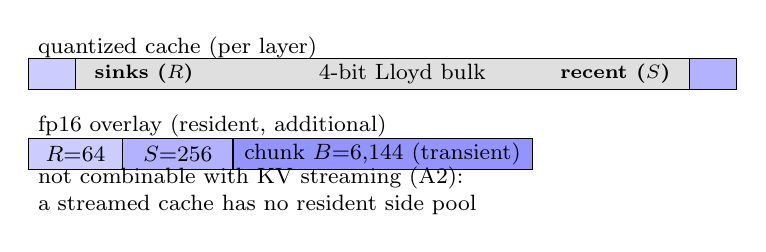
\begin{tikzpicture}[every node/.style={font=\footnotesize},x=1cm,y=0.55cm]
  % main quantized cache bar
  \node[anchor=west] at (0,3.35) {quantized cache (per layer)};
  \draw[fill=gray!25] (0,2.4) rectangle (9.0,3.1);
  \node at (4.75,2.75) {4-bit Lloyd bulk};
  % which token positions the overlay additionally covers:
  % sinks at the START of the cache, recent cells at its end.
  % The cells themselves stay quantized in the base (overlay is additional).
  % Sliver widths are exaggerated; position order is exact;
  % sliver colors match the overlay segments below (no connectors drawn).
  \draw[fill=blue!20] (0,2.4) rectangle (0.6,3.1);
  \draw[fill=blue!30] (8.4,2.4) rectangle (9.0,3.1);
  \node[anchor=west, font=\scriptsize\bfseries] at (0.72,2.75) {sinks ($R$)};
  \node[anchor=east, font=\scriptsize\bfseries] at (8.28,2.75) {recent ($S$)};
  % fp16 overlay bar
  \node[anchor=west] at (0,1.55) {fp16 overlay (resident, additional)};
  \draw[fill=blue!20] (0,0.55) rectangle (1.2,1.25);
  \node at (0.6,0.9) {$R{=}64$};
  \draw[fill=blue!30] (1.2,0.55) rectangle (2.6,1.25);
  \node at (1.9,0.9) {$S{=}256$};
  \draw[fill=blue!42] (2.6,0.55) rectangle (6.4,1.25);
  \node at (4.5,0.9) {chunk $B{=}6{,}144$ (transient)};
  % streaming note
  \node[anchor=west, align=left] at (0,0.05)
    {not combinable with KV streaming (A2):\\ a streamed cache has no resident side pool};
\end{tikzpicture}%
}
\caption{Cache anatomy per layer. The blue slivers mark \emph{which} token positions
the resident fp16 overlay additionally covers --- sinks at the cache's start, recent
cells at its end; sliver widths are exaggerated, the position order is exact, and the
sliver colors match the overlay segments in the second bar. The cells themselves
remain quantized in the 4-bit base; the copied fp16 rows form an \emph{additional}
side pool, not a hole in the cache.}
\label{fig:anatomy}
\end{figure}

\subsection{Operating point}

The production point is $S{=}256$, $R{=}64$ and the automatic prompt chunk capped at $B{=}6{,}144$. Table~\ref{tab:footprint} compares it with the default. The window costs 0.79 bit/cell more than the plain 4-bit base (4.50 bit, 864\,MiB) and frees 36\% of the KV memory against \texttt{int8}.

\begin{table}[t]
\centering
\small
\begin{tabular}{@{}lcc@{}}
\toprule
\textbf{KV mode} & \textbf{Bits/cell} & \textbf{KV at 128K} \\
\midrule
\texttt{int8} (default) & 8.25 & 1,584\,MiB \\
plain \texttt{q4lm8v} & 4.50 & 864\,MiB \\
\texttt{q4lm8v} + window 256/64 & 5.29 & 1,016\,MiB \\
\bottomrule
\end{tabular}
\caption{KV footprint at 128K (131,072 token positions, the 12 full-attention QSA layers of the hybrid model; Section~3). \texttt{int8} stores 8-bit content plus block scales; its 8.25 is the effective rate. The window figure includes the resident ring at $B{=}6{,}144$; the plain figure is from the byte model.}
\label{tab:footprint}
\end{table}

\subsection{Window geometry and cost}

The 4-bit base stores K at 16 levels and V at 8 levels in 18-byte blocks, 576\,B per cell and layer. The window keeps a side copy of the sink and recent cells in fp16. The side copy is \emph{additional} to the quantized row, not a replacement: the exact cell is 16 bits, not $16-\text{base}$ bits. The resident ring holds $R$ sink rows, $S$ recent rows and $B$ rows for the current prompt chunk, so the marginal cost of a windowed run is
\begin{equation}
\text{bits/cell} \;\approx\; 4.50 \;+\; \frac{16\,(R+S+B)}{L},
\end{equation}
where $L$ is the context length in cells. All three terms are resident memory: the ring is sized for the prompt chunk, so the $B$ term dominates the per-cell average at this $L$ ($0.75$ of the $0.79$ added bit/cell at 128K). At 128K with $R{=}64$, $S{=}256$ and $B{=}6{,}144$ this gives 5.29 bit/cell and 1,016\,MiB.

The chunk $B$ follows \texttt{-{}-prefill}. A larger automatic chunk would need a larger ring, and the host's ring batch cap (\texttt{kKvWinBatchMax}) is 6,144 cells, so a windowed run caps the automatic chunk there and says so. A ring the user sizes explicitly is left alone; a chunk that does not fit is refused loudly. The break-even against \texttt{int8} is about 28K cells: solving $16\,(R{+}S{+}B)/L = 8.25 - 4.50$ gives $L \approx 27{,}600$ at $B{=}6{,}144$, and at 32K the window is still cheaper than \texttt{int8} (7.67 against 8.25 bit/element\,\cite{strata-wp}). Setup offers the window only from 32K upwards --- above the break-even, where the memory direction is the right one.

The exact cells must stay resident. A streamed KV cache has no always-resident side pool, so the window and KV streaming do not combine (A2). The window is also orthogonal to the level table: it can be enabled on other 4-bit modes, but the production point is \texttt{q4lm8v} with 256/64.

\section{Design Alternatives Considered}\label{sec:alternatives}

None of the alternatives in this section was measured on this engine. The section records why each was left out; the reasoning is static analysis, not measurement, and every item is a candidate follow-up arm.

\paragraph{Per-channel key quantization.} KIVI and KVQuant quantize K along the channel axis because the key error concentrates in outlier channels~\cite{kivi,kvquant}. Strata's base quantizes per cell after an orthonormal Hadamard rotation, which spreads that outlier energy across channels; whether the rotation makes the cheaper per-cell axis competitive with the per-channel axis on this model is exactly the unmeasured question. It would change the block writer and reader, not the window.

\paragraph{Pre-RoPE key quantization.} KVQuant quantizes K before the rotary positional embedding, because the rotation multiplies the quantization error~\cite{kvquant}. Strata's Hadamard rotation is also pre-quantization; whether the engine's K path can quantize before RoPE instead of after is a kernel-layout question that has not been examined.

\paragraph{Non-uniform levels.} KVQuant derives sensitivity-weighted datatypes~\cite{kvquant}; our K uses 16 uniform Lloyd levels and V uses 8. Non-uniform levels are orthogonal to the window and would change the level tables only.

\paragraph{Low-rank plus sparse correction.} GEAR keeps a correction term for the residual error~\cite{gear}. The window's fp16 overlay is a dense-but-local correction: full 16-bit precision on the ring's cells. A distributed low-rank correction would cover the whole cache at a smaller byte rate, at an added latency cost; both would need new kernel shapes.

\paragraph{Layer-wise precision pairs.} KVTuner reaches a nearly lossless 3.25-bit point with different precision per layer~\cite{kvtuner}. Strata's KV format is global per cache; per-layer level tables are representable in the block layout but add configuration space that setup would have to explain to users.

\paragraph{Eviction on top of the 4-bit base.} SnapKV/H2O-style eviction is a larger memory win with a different cost: cells leave the cache~\cite{snapkv,h2o}. The window keeps the whole context addressable --- the A-series treats a silently unavailable exact cell as a fault --- so eviction is out of scope for this point; a combined mode would be a separate opt-in with its own hardening.

\paragraph{A streaming-compatible sink pool.} A2 refuses the window under streaming. A tiny sink-only side pool ($R$ cells, no recent ring) could in principle combine with a streamed cache, because sinks never scroll far from position~0. We did not build it: the sink budget interacts with the streaming host copy, and the contract prefers loud refusal over a new silent-failure surface. Untested.

\section{Hardening: Preventing Silent Failures}

The guiding principle is that a silent misread is worse than a loud refusal. When the window cannot guarantee an exact read, it should stop, refuse the configuration, or fail an invariant---not fall back quietly to a quantized value that the caller believes is exact. Table~\ref{tab:decisions} summarizes decisions A1--A5, including A4 as the visible open item.

\begin{table*}[t]
\centering
\small
\begin{tabularx}{\textwidth}{@{}l >{\raggedright\arraybackslash}X >{\raggedright\arraybackslash}X >{\raggedright\arraybackslash}X@{}}
\toprule
\textbf{ID} & \textbf{Observed problem} & \textbf{Decision} & \textbf{Evidence} \\
\midrule
A1 & The automatic prompt chunk could exceed the ring's batch cap, so an append in the middle of a long prompt aborted the run. & Cap the automatic chunk at the ring's batch maximum (6,144) when the window is active and the user did not set a size; cover the generate and serve paths. & The pre-fix failure is the logged one (an 8,191-token prompt, \texttt{-{}-prefill auto:16384}, aborted); post-fix completion is the capped path's behavior (static reading of \texttt{generate.cpp}). An explicitly undersized ring is still refused. \\
A2 & Setup could write a streamed KV cache beside the window. A streamed cache has no always-resident side pool, so a promised exact read could silently become quantized. & Setup never writes the pair and explains why; the engine refuses the pair before loading anything. & The pair is refused before load with exit code~2; window alone and \texttt{int8} with streaming both run\,\cite{strata-details}. \\
A3 & The $(S,R,B)$ grid could drift between the main state and a later-carved MTP/twin state. Different grids on the same contract are incorrect. & Freeze the grid after the prompt chunk and assert stability on later batch changes. & The grid stays stable; the default logits SHA is unchanged. The check is a debug assert (release builds warn and continue); probe results are not in the measurement history. \\
A4 & The window's write/read paths have no full parity test across all shapes, so a shape-specific misread would be silent. & \textbf{Open item.} Dump every window row at write time and re-read it through the window reader on every shape: ring wrap, stale tags, sinks, batch boundaries, empty tags. & Not yet run; the test is specified in the repository and is a review gate. \\
A5 & Zero-initialized ring rows were tagged as cell~0 and could be read as a valid exact cell. & Initialize empty tags to a sentinel; a stale or mismatched tag falls back to the quantized row. & Empty-state semantics are correct and the default path is unchanged. \\
\bottomrule
\end{tabularx}
\caption{Hardening decisions A1--A5. The A4 row is the open follow-up item (a full cell-to-row parity test across all shapes), a review gate rather than a shipped fix.}
\label{tab:decisions}
\end{table*}

Two decisions deserve emphasis. A2 is enforced twice---once in setup, where most users will meet it, and once in the engine, where a hand-edited configuration can still arrive. A3 is deliberately a freeze-and-assert rather than a full state-layout refactor; the assert is active in debug builds, and a release build prints a warning and continues. A4 is the one item in the A-series that is still open.

\section{Evaluation Methodology}

\subsection{Corpora}

Three fixed teacher-forced corpora are used. The 2K set is the RULER \emph{complex word extraction} task in eight contiguous segments, 16,351 scored positions. The 4K set uses the same task with eight segments of 4,096 tokens, 32,746 positions. The 128K set is two texts from the same generator (same seed, alpha and 2,621 code words, drawn separately)\,\cite{strata-details}; the first is one 131,063-token segment, 131,062 scored positions, scored on the last 4,096 positions and on the whole segment, and the second is scored on the same regions (Section~7.3). The three sets are different texts; numbers are not comparable across lengths, and the 4K set is not a length-scaling experiment for the 128K set.

\subsection{Reference and scoring}

The reference is fp16 K/V with fixed Swift~1.5 IQ3\_XXS weights. The model is given the reference text and the log-probabilities are read; there is no free generation. Each arm is a separate engine run, and the harness records per-position log-probabilities and compares them offline, so KL, top-1 and PPL come from the same pass. The KV cache of the prefill is quantized along with the decode cache, so the absolute gaps are internal Strata numbers and are not directly comparable with field numbers measured decode-only. Each quality run uses one expert slot and \texttt{-{}-prefill 512} on all three corpora, and the text is scored through \texttt{-{}-short-read} (one decode step at a time, so a scored token's exact set is the $R{+}S$ overlay, not the production chunk). The batched $B{=}6{,}144$ prefill was not quality-scored; that it scores the same is a static argument, not an A/B\,\cite{strata-wp}. The runtime runs use the automatic expert cache and a mixed prompt set.

\subsection{Metrics}

Four metrics are reported. \emph{Mean KL} is the Kullback--Leibler divergence $D_{\mathrm{KL}}(p_{\mathrm{ref}}\,\|\,p_{\mathrm{arm}})$, from the fp16 reference distribution to the arm's distribution, in nats per position; zero means identical, and lower is better. As the harness computes it for these tables, the KL is truncated to the reference's 64 most likely tokens: both distributions are renormalized onto that set, and a token the arm's own 64-token list omits contributes the arm's 64th log-probability as a floor\,\cite{strata-quants}. This is not the KL of the two full next-token distributions --- mass outside the reference's top-64 enters only through the floor --- and the numbers here are comparable only within this definition. The direction penalizes an arm that puts little probability mass where the reference has mass, which is the kind of error a downstream sampler inherits; mass the arm places on its own private modes is invisible to it. The reverse direction, a full-vocabulary rescore (which would be a new scoring pass), and the truncation boundary itself were not measured; the ranking could differ under any of them. \emph{p99 KL} is the 99th percentile of the per-position KL under the same truncated definition: it exposes a heavy error tail that a good mean can hide, and the isolated 17-nat positions of Table~\ref{tab:regions} carry a floor's signature --- the arm's top-64 list missing a reference mode --- so they should not be read directly as full-distribution events. \emph{Top-1} is the fraction of positions where the arm's argmax equals the fp16 argmax; it is a coarse agreement measure, not target accuracy. \emph{Perplexity} is $\exp$ of the mean negative log-likelihood of the true tokens. Perplexity is reported for context only: quantized-KV error tends to damp the distribution, so a quantized arm can score \emph{below} the fp16 reference while its $D_{\mathrm{KL}}(p_{\mathrm{ref}}\,\|\,p_{\mathrm{arm}})$ is positive. KL, not perplexity, is the decision metric. The p99 entries are point estimates; at these position counts their sampling error is much smaller than the spread between arms, but it is not quantified here --- a bootstrap over positions (computed on this truncated KL) is the cheapest missing piece and needs no new runs.

\subsection{Paired statistics}

Both arms see the same positions. We compute the KL difference per segment, then average over the eight segments. The text cancels, so the spread is much smaller than in a comparison of two independent means. We report the paired $t$ statistic and the number of segments whose difference carries the stated direction, which each result names explicitly. With eight segments (seven degrees of freedom), $|t|\gtrsim2.4$ is roughly $p<0.05$ two-sided and $|t|\gtrsim3.5$ roughly $p<0.01$. A large $t$ with an unfavorable sign count is not a result; the sign count is read alongside every headline number. The 128K set is one segment, so its eight 4K blocks are adjacent and not independent; its $t$ is a rough reading, not a segment-pair test.

\subsection{Runtime, memory and correctness gates}

Runtime is a same-day A/B with a fresh server per arm and two alternating rounds; the engine's own prefill and decode counters are read, and table entries are medians of the two rounds. The reported runs use a mixed prompt set --- short and long prompts over the same serving session --- whose per-prompt results are documented in the measurement report\,\cite{strata-wp}; the hit rate column is the expert-cache hit rate over that set (the fraction of expert lookups served from the resident cache). Reported memory is KV bytes at 128K and resident expert slots. The correctness gate is byte-identity: the \texttt{int8} default's dump-logits SHA must be identical across runs, and every window change must leave it unchanged. Targeted probes reproduce the former crash and the refusal cases; kernel parity tests compare the window writer and reader bitwise; needle tests at 32K and 128K check that retrieval does not regress.

\subsection{Provenance and reproducibility}

Every number in this paper is traceable to the repository's measurement history: the window work --- the 2K/4K quality tables, the runtime A/B and the first 128K text --- is documented in \texttt{docs/KV\_QUANT\_WORKPACKAGE.md}\,\cite{strata-wp}, the authoritative byte model and quality section in \texttt{docs/DETAILS.md}\,\cite{strata-details}, and the plain-4-bit document-perplexity measurement in \texttt{bench/results/2026-09-27-kv-q4}\,\cite{strata-kv4}. The cwe corpora are RULER complex-word-extraction texts generated by the repository's quant-quality harness (fixed segment structure and scored positions per section above); the harness records the per-position log-probabilities the statistics are computed from. No new runs were produced for the quality tables; where a figure is byte-model rather than runtime-observed, the table captions say so. The one run added for this revision is the 2026-10-24 needle pair (Section~7.5); its JSON and engine logs (\texttt{.txt}; \texttt{*.log} is gitignored) are in the tree\,\cite{strata-needle24}. Two provenance limits are named rather than smoothed over. First, the workpackage runs behind Tables~\ref{tab:runtime}--\ref{tab:regions} used engine build 0.1.44.1, while \texttt{DETAILS.md} was written under a 0.1.47 Windows--HIP build; it carries the first text's tail numbers to the printed digit plus the second 128K text, whose raw per-position log is not in the tree (Section~7.3). Second, \texttt{docs/QUANTS.md} documents the top-64 KL convention for the weight-quantization yardstick, not the cwe protocol, and the window's raw \texttt{bench/results} directories hold no logs in this tree --- the workpackage on that branch is the report.

\section{Results}

\subsection{Memory and speed}

Table~\ref{tab:runtime} gives the 128K runtime point. The production arm (256/64, $B{=}6{,}144$) has the same prefill throughput as \texttt{int8}, decode 1.0 token/s lower with changing signs across rounds (inside the run-to-run spread), and frees 568\,MiB of VRAM at 128K, which the expert cache converts into 416 more resident expert slots and a slightly higher hit rate. These are capacity figures, not speed wins: serving throughput at concurrency was not measured. The $B{=}512$ arm is cheaper (4.60 bit, 884\,MiB) but prompts at 105 token/s, about five times slower, so it is an offline/batch point. The 512/128 arm is not chosen: at 4K its quality is statistically identical to 256/64 (paired $t{=}{+}0.02$, Table~\ref{tab:q4k}), it was not quality-scored at 128K, it costs 7\,MiB more (Table~\ref{tab:runtime}), decodes about 0.85 token/s slower, and its apparent prefill advantage did not reproduce on the needle prompts.

\begin{table*}[t]
\centering
\small
\begin{tabular}{@{}lcccccc@{}}
\toprule
\textbf{Arm} & \textbf{Bit} & \textbf{MiB} & \textbf{Slots} & \textbf{Prefill} & \textbf{Decode} & \textbf{Hit} \\
\midrule
\texttt{int8} & 8.25 & 1,584 & 3,033 & 526.1 & \textbf{35.2} & 0.74 \\
256/64, $B{=}6{,}144$ & 5.29 & 1,016 & 3,449 & 528.0 & 34.2 & 0.76 \\
256/64, $B{=}512$ & \textbf{4.60} & \textbf{884} & 3,496 & 105.0 & 34.5 & 0.76 \\
512/128, $B{=}6{,}144$ & 5.33 & 1,023 & 3,412 & \textbf{634.0} & 33.35 & 0.77 \\
\bottomrule
\end{tabular}
\caption{128K runtime (Swift~1.5 IQ3\_XXS, RX~9060~XT 16\,GB, Windows HIP; engine build 0.1.44.1, \texttt{-{}-spec 4} MTP drafting on). Prefill and decode in tokens/s; decode is the serving rate under drafts, so the spread includes draft acceptance, not only the KV format. Medians of two same-day alternating rounds over a mixed prompt set. The 512/128 prefill advantage did not reproduce on the needle prompts and is shown for completeness.}
\label{tab:runtime}
\end{table*}

\subsection{Quality at 2K and 4K}

Tables~\ref{tab:q2k} and~\ref{tab:q4k} report the short-context quality; all quality statements in this section are for the cwe task and this model, and are not length-scaling claims across the different corpora. At 2K the window's mean KL is 0.00702 against \texttt{int8}'s 0.00503, but the paired difference is not significant ($t=-1.92$ in \texttt{int8}'s favor; the window is ahead in only 2 of the 8 segments). The window is also close in the tail: p99 0.0835 against 0.0733. It removes most of the plain 4-bit arm's error (0.01791) and lands near \texttt{int8}.

At 4K \texttt{int8} is significantly better on the mean (0.01688 against 0.02090; paired $t=-3.55$, and 7 of the 8 segments favor \texttt{int8}), and the window closes 73\% of the plain-arm-to-\texttt{int8} gap ($0.01093/0.01494$). In the small answer region the two are not distinguishable ($t=-0.51$; descriptive, small region). The 512/128 form is statistically identical to 256/64 ($t=0.02$), so the smaller form is kept.

\begin{table}[t]
\centering
\small
\begin{tabular}{@{}lcccc@{}}
\toprule
\textbf{Arm} & \textbf{Top-1} & \textbf{Mean KL} & \textbf{p99 KL} & \textbf{PPL} \\
\midrule
fp16 (reference) & --- & 0 & --- & 2.999 \\
\texttt{int8} & 99.35\% & \textbf{0.00503} & \textbf{0.0733} & 3.004 \\
plain \texttt{q4lm8v} & 98.92\% & 0.01791 & 0.2793 & 3.024 \\
+ window 256/64 & 99.33\% & 0.00702 & 0.0835 & 3.003 \\
+ window 512/128 & \textbf{99.39\%} & 0.00623 & 0.0743 & \textbf{2.995} \\
\bottomrule
\end{tabular}
\caption{Quality on cwe-2k (16,351 positions, fp16 K/V reference). Top-1 is agreement with the fp16 argmax; KL in nats/position.}
\label{tab:q2k}
\end{table}

\begin{table}[t]
\centering
\small
\begin{tabular}{@{}lcccc@{}}
\toprule
\textbf{Arm} & \textbf{Top-1} & \textbf{Mean KL} & \textbf{p99 KL} & \textbf{PPL} \\
\midrule
\texttt{int8} & \textbf{99.05\%} & \textbf{0.01688} & \textbf{0.1888} & 2.860 \\
plain \texttt{q4lm8v} & 98.40\% & 0.03182 & 0.5785 & 2.888 \\
+ window 256/64 & 98.84\% & 0.02090 & 0.2811 & 2.858 \\
+ window 512/128 & 98.95\% & 0.02088 & 0.2822 & 2.858 \\
\bottomrule
\end{tabular}
\caption{Quality on cwe-4k (32,746 positions). cwe-4k is a different text from cwe-2k; the two tables are not comparable across sets.}
\label{tab:q4k}
\end{table}

\subsection{Quality at 128K}

Table~\ref{tab:q128k} reports the tail of the \emph{first} 128K text, and Table~\ref{tab:regions} the other regions. On the last 4,096 positions the window's mean KL is 0.00663 against \texttt{int8}'s 0.00959, a 31\% lower mean, but the paired eight-block $t$ is $-0.74$: the lead is not significant and comes from two blocks in which \texttt{int8} has its own spikes. The robust reading favors \texttt{int8}: it has the better p99 (0.01655 against 0.02977), the better last 1,024 positions (0.00265 against 0.00444), and the better whole segment (0.10715 against 0.13312); the region table also shows a lower answer-region KL for \texttt{int8}, but that region has 27 positions, so the number is descriptive only and we do not use it as an argument. The window still beats the plain 4-bit base clearly: mean KL 0.00663 against 0.01587 (58\% lower), whole segment 0.13312 against 0.15758, and p99 0.0298 against 0.0308. The 128K result is therefore the same story as 4K: the window recovers much of the base's loss and approaches \texttt{int8}, but does not overtake it.

\textbf{The second text.} The 128K generator produced two texts (same seed, alpha and 2,621 code words, drawn separately); the second --- printed in \texttt{DETAILS.md} but not in the workpackage's quality block --- changes the tail story\,\cite{strata-details}. On its last 4,096 positions \texttt{int8} wins the mean (0.00324 against the window's 0.00437; plain 0.00664) and the p99 (0.0165 against 0.0210); here the window closes 34\% of the plain arm's tail KL rather than 58\%, and \texttt{int8} also wins the whole segment (0.06435 against 0.07524 and plain 0.08834). Stable across both texts: the window clearly beats the plain 4-bit base and \texttt{int8} wins the whole segment; the gap between the two quantized arms is not consistent even in sign, which is why the robust reading rests on the p99, the last 1,024 positions and the whole segment rather than on the tail mean. Provenance caveats: \texttt{DETAILS} reports the first text's tail under its 0.1.47 build label with the digits of the workpackage's 0.1.44.1 table (rerun or retold is not recorded), and the second text's raw per-position log is not in the tree, so its numbers stand as a reported reading, not a re-runnable table.

\begin{table*}[t]
\centering
\small
\begin{tabular}{@{}lcccccc@{}}
\toprule
\textbf{Arm} & \textbf{Bit @128K} & \textbf{KV MiB} & \textbf{Mean KL} & \textbf{p99 KL} & \textbf{Top-1} & \textbf{PPL} \\
\midrule
\texttt{int8} & 8.25 & 1,584 & 0.00959 & \textbf{0.01655} & \textbf{99.73\%} & 2.4052 \\
256/64 & \textbf{5.29} & \textbf{1,016} & \textbf{0.00663} & 0.02977 & \textbf{99.73\%} & 2.4079 \\
plain \texttt{q4lm8v} & 4.50 & 864 & 0.01587 & 0.03079 & 99.51\% & 2.4029 \\
\bottomrule
\end{tabular}
\caption{Quality on the \emph{first} cwe-128k text (Section~7.3), last 4,096 positions (context 126,967--131,062). The fp16 reference has KL~0 and PPL~2.4149; target-token top-1 is 79.74\%. This p99 covers the tail region only and is not comparable with the whole-corpus p99 of Tables~\ref{tab:q2k} and~\ref{tab:q4k}; over the whole 128K segment the p99 is 3.66--5.55 at all three arms (Table~\ref{tab:regions}), driven by isolated hard positions. The 864\,MiB of the plain arm is from the byte model, not a runtime reading.}
\label{tab:q128k}
\end{table*}

\begin{table}[t]
\centering
\small
\begin{tabular}{@{}lccc@{}}
\toprule
\textbf{Region / metric} & \texttt{int8} & 256/64 & plain \\
\midrule
Last 1,024, mean KL & \textbf{0.00265} & 0.00444 & 0.01096 \\
Last 1,024, p99 KL & \textbf{0.04056} & 0.06283 & 0.13641 \\
Whole segment, mean KL & \textbf{0.10715} & 0.13312 & 0.15758 \\
Whole segment, p99 KL & \textbf{3.65623} & 4.75603 & 5.55046 \\
Answer region (27), mean KL & \textbf{0.00526} & 0.00861 & 0.01155 \\
Answer region, top-1 & \textbf{96.30\%} & 92.59\% & \textbf{96.30\%} \\
\bottomrule
\end{tabular}
\caption{First cwe-128k text by region (Section~6.2's \texttt{-{}-short-read} path). The KL rows are fp16-reference KL; \emph{the top-1 row is target-token accuracy, not the fp16-argmax agreement of Table~\ref{tab:q128k}}, and is computed over 27 positions: $25/27=92.59\%$, $26/27=96.30\%$ --- a difference of one position, not a result. The whole-segment p99 values are dominated by isolated hard positions (the measurement report lists single-position KLs of 17.3, 17.1 and 15.8); \texttt{int8} reaches 3.66 as well, so they do not separate the arms.}
\label{tab:regions}
\end{table}

\subsection{Reading the results}

Three conclusions follow, all within this task family and this model. First, the window does what it was designed to do: it removes most of the plain 4-bit base's error at every length tested, and at 2K it is statistically indistinguishable from \texttt{int8} on cwe-2k. Second, it does not replace \texttt{int8} as the quality default. At 4K \texttt{int8} is significantly better on the mean; at 128K it keeps the p99, the last 1,024 positions and the whole segment on both texts, while the tail mean favors each quantized arm on one text (inside the text-to-text spread). The window saves 36\% of the KV memory at the price of a small, measurable quality gap that the mean KL alone can hide. Third, perplexity is not a useful discriminator here: the 128K PPL values (2.4052, 2.4079, 2.4029) all sit below the fp16 reference (2.4149) while every KL is positive. Reporting PPL without KL would reverse the ranking.

\subsection{Correctness gates}

The default path is unchanged: the \texttt{int8} dump-logits SHA (\texttt{A014F504\ldots BA052}) is byte-identical to the pre-window release for \texttt{-{}-kv int8} and \texttt{-{}-kv fp16}\,\cite{strata-details}. The former crash config now completes under the 6,144 cap (the failure is the logged pre-fix one; the completion is the capped path's behavior, Table~\ref{tab:decisions}); an explicitly undersized ring is still refused; the window-plus-streaming pair is refused before loading anything with exit code~2. Kernel parity tests pass 12/12, and the workpackage needle gate is 18/18 at 32K and 128K (6/6 on plain, 256/64 and 512/128; saturated, no regression and no separation)\,\cite{strata-wp}. On 2026-10-24 the production pair was asked again, engine 0.1.47, same card, Swift~1.5 IQ3\_XXS, \texttt{-{}-spec 4}, chunk 6,144: \texttt{int8} and the 256/64 window, the same six needles (32K and 128K, depths 10/50/90\%, one code word, greedy). Both found 6/6, and each answer is the planted word\,\cite{strata-needle24}. Still saturated: no regression, no separation, and not a stand-in for the three-arm gate. A full cell-to-row parity test remains open (A4).

\section{Discussion: Where the Point Fits}\label{sec:discussion}

\subsection{A decision rule}

The measured numbers compose into a short rule for operators. If the context sits below the roughly 28K-cell break-even, the ring costs more than the 4-bit base saves (Section~3.2); setup offers the window from 32K, where it is still cheaper than \texttt{int8} (7.67 against 8.25 bit/element). At long context, quality-first workloads keep \texttt{int8}: it wins or ties every whole-segment statistic that carries weight on both 128K texts, and every region statistic at 2K and 4K (Tables~\ref{tab:q2k}--\ref{tab:q128k}). Memory-bound workloads at 128K take the window: 568\,MiB freed, 416 more resident expert slots, prefill parity, decode inside spread (Table~\ref{tab:runtime}), and a measured KL penalty that is small on this task family and bounded by the 4K and 128K readings. Setup already follows this shape: \texttt{int8} is the default, the window is opt-in from 32K upwards.

\subsection{How firm is the grid}

The neighborhood of the production grid is measured more thinly than the endpoints. On cwe-2k the production sink depth ($R{=}64$, $S{=}256$) is already statistically indistinguishable from \texttt{int8} on both level-table bases\,\cite{strata-wp}; the knee near $S{=}512$ sometimes quoted from the earlier rounds sits on the thinner $R{=}8$ arms of the 16-level base and must not be read as a statement about the shipped grid. At 4K the 512/128 pair scores the same quality as 256/64 (paired $t{=}{+}0.02$, Tables~\ref{tab:q2k} and~\ref{tab:q4k}) for 7\,MiB more and a slower decode, which is why 256/64 ships; at 128K the 512/128 grid was not quality-scored, so there is no quality statement for it there. What was not measured at 128K is anything smaller than 256/64: the shipping decision rests on the 4K quality tie plus the 128K runtime A/B, and on 256/64 being the cheapest 128K arm with a clean quality reading, not the local optimum. A finer sweep of $S$ and $R$ at 128K --- and the knee move observed at 2K, where the load-bearing $S$ sits higher --- is the natural next measurement.

\subsection{Cheaper overlays exist on paper}

The window is orthogonal to the level table, and the workpackage trialed thinner level tables on the same mechanism early on\,\cite{strata-wp}. Under the corrected byte model and the production sink depth the early reading shrinks: at the original $R{=}8$ sink depth on cwe-2k, the then-current byte model put a crossover near 4.8--5.3 bit/element where an 8-level-V windowed base looked byte-competitive; that crossover was withdrawn as an artifact of the too-small sink count (at $R{=}64$ the two bases were not separable across five shapes, $|t| \le 1.5$), and the old byte model itself was superseded (the exact cell is additional; the span is $R{+}S{+}B$). What survives is that the window carries shorter level tables without measurable cost at $R{=}64$. A $\leq$3-bit base at 128K --- the same mechanism at even fewer bytes --- is unmeasured and is a concrete follow-up arm; its byte side must be priced with the corrected model.

\subsection{Two unmeasured workload questions}

Two questions bound how the point is used today. First, multi-turn growth: the window's home workload is a chat that grows by small appends to a long context, every turn after the first presumably reading large parts of the cache; the quality runs here score single segments, and the runtime A/B's mixed prompt set is the only evidence for repeated prompting. Second, mid-context degradation: the 128K corpus is scored at the tail, and the 4K corpus shows that per-cell quantization hurts where nothing protects the cell. A one-arm interior reading exists --- the workpackage reports, for the window arm, KL 0.054 on the first 4,096 positions and 0.164 on one middle 4K block (positions 65,536--69,631)\,\cite{strata-wp} --- but the other arms are not scored on that block, so the paired mid-segment comparison is unmeasured. The first question is unmeasured outright. Neither argues for removing the window, but both belong on the list before larger deployment claims.

\section{Threats to Validity}

The measurements come from one GPU (RX~9060~XT, gfx1200), one operating system (Windows), one ROCm/HIP stack (7.1) and one weight set (Swift~1.5 IQ3\_XXS); the tables name the engine build that produced them (Section~6.6). CUDA and SYCL were not built; the changes are backend-agnostic, but that is an argument, not a measurement. The short-context results have eight segments; each 128K result is one text with adjacent blocks, so those $t$ values are descriptive. The $R{+}S{+}B$ ring is 20.3\% of the 4K context at $B{=}512$ and 4.9\% of the 128K context at $B{=}6{,}144$; those are the ring's resident capacity. A scored token under the short-read quality path sees the $R{+}S$ overlay (320 positions\,\cite{strata-wp}), of which only the cells the indexer selects are read exact (Section~3, static reading); the 4K KL is an upper bound on the long-context benefit, not a prediction, and the 128K KL is measured separately. The prefill KV is also quantized, so the absolute KL gaps are not comparable with decode-only field numbers. Finally, the window is a memory trade-off, not a quality improvement over \texttt{int8}; the paper should be read that way. Two coverage limits stand out. The quality evidence comes from one task family (RULER complex word extraction) on one model; the full RULER set or LongBench subsets were not run, so the quality sentences here carry no claim outside this family. And no community-standard arm --- for example a KIVI-style per-channel-K quantization with an fp16 residual~\cite{kivi,kvquant} --- was measured on this engine, so the 5.29-bit point has no external anchor on the published trade-off curve; the fair version of that arm is per-channel before the rotation, on this indexer-architecture cache, not on a dense-attention cache (Section~\ref{sec:followup}). One intermittent engine hang was seen once on the \emph{plain} 4-bit arm (no window) during a 128K prefill; it did not reproduce in 6/6 reruns, and the window arms completed three 128K runs without it --- an open engine bug report, not evidence against the window.

\section{Avenues for Improvement}\label{sec:followup}

The sections above are the status quo. The window does not beat \texttt{int8} on the statistics that carry weight, and a larger window is not how that changes. It spends the byte headroom, from 5.29 toward 8.25 bit/cell, on more exact cells and leaves the bulk at 4 bits, where \texttt{int8} is the better code. Under a ceiling of 6.0 bit/cell at most 9\% of the cells can be exact (the exact side copy costs 16 bit/cell and the 4-bit row it duplicates stays), and the 512/128 pair already ties 256/64 at 4K while doubling the exact overlay (Section~8.2). The package below is a falsification ladder. Nothing in it is a result.

Two bars apply, and they answer different questions. \textbf{Bar~A asks whether a new mode is worth shipping as an opt-in.} The paired 4K mean KL stays within $+0.002$ nats of \texttt{int8} (the current window sits at $+0.00402$), the 128K whole segment and p99 stay within $+0.013$ and $+0.007$ on both texts (the current window sits at $+0.02597$ and $+0.01322$ on its worse text), the effective rate stays at or below 6.0 bit/cell, and the correctness gates stay green. At 6.0 bit/cell the byte model gives about 1,152\,MiB at 128K against \texttt{int8}'s 1,584\,MiB --- about 432\,MiB, or 27\%, less, linear between the two measured points of Table~\ref{tab:runtime}. The margins are choices, not measurements: each is half of today's measured gap, and the raw numbers are reported either way. A mode that meets Bar~A replaces the current opt-in point and leaves the default alone.

\textbf{Bar~B asks whether the default should move}, and it is the bar the conclusion refers to. An arm wins only if four things hold, all set before the first new run. Paired mean KL at 4K does not favor \texttt{int8}. Whole-segment KL and p99 at 128K do not favor \texttt{int8} on either text. The effective rate at 128K stays under 8.25 bit/cell; otherwise the result is to keep \texttt{int8}. The \texttt{int8} dump-logits SHA is unchanged. A tie is not a win. A tail-mean win on one text is not a win: the window already has one, and it reverses on the second text. A 128K run is not started for an arm that has not won at 4K. Every arm is opt-in.

The work package has already closed five doors, and this package does not reopen them\,\cite{strata-wp}. Clipping after the rotation made the 2K KL worse. Turning the Walsh--Hadamard off was a tie on the 16-level base at 2K and 4K, which is not a statement about the production window. A K-versus-V bit contrast did not support giving the keys more bits ($t{=}{+}0.05$). A 3-bit base without the window was worse. $R{=}8$ was too small a sink count. The published direction that keys should keep the bits\,\cite{spectralkv} stands as their result on their models. It is not a reason to rerun a contrast this model has already failed.

Each step has a kill, and the next step starts only if the kill did not fire.

\begin{enumerate}
\item Rescore one existing 4K pair under a wider KL than the top-64 truncation of Section~6.3. Scorer only; the engine is not touched. If the ranking and the sign count agree with Table~\ref{tab:q4k}, the bar stands. If they flip, no kernel is built until 128K is reread under the same definition.
\item Count, on one 128K prefill, the share of indexer selections that fall in $R$, in $S$, and in neither. The rule, set now, is that a share below one half in $R{+}S$ kills a larger positional window. The sink-and-recent overlay is then the literature's mechanism\,\cite{kivi,skvq,intactkv,rotatekv} implemented on cells this model does not read. That sentence is a static reading until the counter is run (Section~3).
\item Report channel second moments of K before and after the Walsh--Hadamard, split into the 64 rotated dimensions and the 192 that are not. If the pre-rotation channels are not the heavier tail, a per-channel arm is not built. Per-channel scales after the rotation are not the arm: the rotation mixes the channels (Section~3, static).
\item Run only formats the engine already has: 16 levels on K and on V, plus the production window, against \texttt{int8}, at 4K. A tie kills it. No 128K follows a tie.
\item Build a per-channel scale before the rotation, on the two slices of step 3, only if step 3 did not kill it. Score it at 4K. It is the KVQuant axis\,\cite{kvquant} in the form this geometry allows, not a pre-RoPE port of a fully rotated head.
\item Take a 4K winner to 128K, both texts, whole segment and p99. Ignore the tail mean. A second task family is the check after that win, not the search for it.
\end{enumerate}

Two facts about this model bound which survey methods can be that winner. Only 12 of 48 layers carry this cache; the other 36 keep a fixed recurrent state, so a method that compresses every layer's cache does not apply. And the indexer may later select any stored cell. Dropping cells, or replacing the selection, is not a cache format here: a selected cell that is no longer present is the silent failure the A-series already treats as a fault. Two KV heads leave no room for a retrieval-head split\,\cite{duoattn,razorattn}. Learned rotations, calibrated codebooks and rewritten projections\,\cite{spinquant,palu} are a different model, not an opt-in flag. FP8 is not a kernel this GPU has.

If step 2 says the positional overlay misses the cells that are read, the remaining avenue is to spend the exact bytes on cells the indexer returned and keep every cell addressable at 4 bits\,\cite{top-k}. The selected set changes per query, so the pool is a union or the last selection, and a promised exact cell that has left the pool is the same fault as a dropped cell. That avenue does not start until the counter says the current overlay is in the wrong place.

Two review gates stay beside the ladder, and neither is a quality claim. A full cell-to-row parity test should dump every window row at write time and re-read it on every shape: ring wrap, stale tags, sinks, batch boundaries and the empty tag. CUDA and SYCL should compile and pass their parity suites. \texttt{q4lm8v} is not offered on SYCL, so the window paths are dead there, but they should still compile. The paired mid-segment score and a multi-turn append (Section~8.4) stay on the list. They bound how the current point is used. They are not a path past \texttt{int8}.

\section{Conclusion}

Hardening the exact-cell window was primarily an exercise in preventing silent failures at integration boundaries. Setup-side prevention and engine-side enforcement close the window-plus-streaming hole; a frozen grid closes state drift; sentinel tags close the empty-cell misread; a capped automatic chunk closes the mid-prompt abort. The default \texttt{int8} path stays byte-identical. The measurement-first validation shows the intended trade-off clearly: on the cwe corpora, the window removes most of the 4-bit base's KL error (73\% of its gap to \texttt{int8} at 4K; 34--58\% of the plain base's tail mean KL across the two 128K texts), approaches \texttt{int8} at 2K, and saves 36\% of the KV memory at 128K. It does not beat \texttt{int8} in the tail regions that carry weight --- the p99 and whole-segment numbers say so on both texts. That is the correct result for an opt-in memory point: keep \texttt{int8} as the quality default, offer the window where memory is the constraint, and measure both. Section~\ref{sec:followup} is the package that would have to beat that default, and the kills under which it would be dropped.

Two habits generalize beyond this feature. First, correctness is enforced where the failure would be silent: setup-side for users, engine-side for hand-edited configs, and a byte-identity gate for everything the default path touches. Second, an opt-in point earns its existence only against measured alternatives --- here, against \texttt{int8} in regions that the mean KL alone cannot see. Both habits cost little and transfer to the next integration-boundary feature.

\begin{thebibliography}{34}
\setlength{\itemsep}{0pt}\footnotesize

\bibitem{streamingllm}
G.~Xiao, Y.~Tian, B.~Chen, S.~Han, M.~Lewis.
\emph{Efficient Streaming Language Models with Attention Sinks}.
arXiv:2309.17453, 2023 (ICLR 2024). Code: \url{https://github.com/mit-han-lab/streaming-llm}.

\bibitem{kivi}
Z.~Liu, J.~Yuan, H.~Jin, S.~Zhong, Z.~Xu, V.~Braverman, B.~Chen, X.~Hu.
\emph{KIVI: A Tuning-Free Asymmetric 2bit Quantization for KV Cache}.
ICML 2024, arXiv:2402.02750. Code: \url{https://github.com/jy-yuan/KIVI}.

\bibitem{kvquant}
C.~Hooper, S.~Kim, H.~Mohammadzadeh, M.~W.~Mahoney, Y.~S.~Shao, K.~Keutzer, A.~Gholami.
\emph{KVQuant: Towards 10 Million Context Length LLM Inference with KV Cache Quantization}.
NeurIPS 2024, arXiv:2401.18079. Code: \url{https://github.com/SqueezeAILab/KVQuant}.

\bibitem{gear}
H.~Kang et~al.
\emph{GEAR: An Efficient KV Cache Compression Recipe for Near-Lossless Generative LLM Inference}.
arXiv:2403.05527, 2024.

\bibitem{snapkv}
Y.~Li et~al.
\emph{SnapKV: LLM Knows What You Are Looking for Before Generation}.
NeurIPS 2024, arXiv:2404.14469.

\bibitem{pyramidkv}
Z.~Cai et~al.
\emph{PyramidKV: Dynamic KV Cache Compression based on Pyramidal Information Funneling}.
COLM 2025, arXiv:2406.02069.

\bibitem{h2o}
Z.~Zhang et~al.
\emph{H2O: Heavy-Hitter Oracle for Efficient Generative Inference of Large Language Models}.
NeurIPS 2023, arXiv:2306.14048.

\bibitem{quarot}
S.~Ashkboos, A.~Mohtashami, M.~L.~Croci, B.~Li, P.~Cameron, M.~Jaggi, D.~Alistarh, T.~Hoefler, J.~Hensman.
\emph{QuaRot: Outlier-Free 4-Bit Inference in Rotated LLMs}.
arXiv:2404.00456, 2024.

\bibitem{rotatekv}
Z.~Su, Z.~Chen, W.~Shen, H.~Wei, L.~Li, H.~Yu, K.~Yuan.
\emph{RotateKV: Accurate and Robust 2-Bit KV Cache Quantization for LLMs via Outlier-Aware Adaptive Rotations}.
arXiv:2501.16383, 2025 (IJCAI 2025).

\bibitem{skvq}
H.~Duanmu, Z.~Yuan, X.~Li, J.~Duan, X.~Zhang, D.~Lin.
\emph{SKVQ: Sliding-window Key and Value Cache Quantization for Large Language Models}.
arXiv:2405.06219, 2024.

\bibitem{intactkv}
R.~Liu, H.~Bai, H.~Lin, Y.~Li, H.~Gao, Z.~Xu, L.~Hou, J.~Yao, C.~Yuan.
\emph{IntactKV: Improving Large Language Model Quantization by Keeping Pivot Tokens Intact}.
ACL Findings 2024, arXiv:2403.01241.

\bibitem{pmkvq}
T.~Liu, S.~Li, J.~Yang, T.~Zhao, F.~Zhou, X.~Song, G.~Dai, S.~Yan, H.~Yang, Y.~Wang.
\emph{PM-KVQ: Progressive Mixed-precision KV Cache Quantization for Long-CoT LLMs}.
ICLR 2026, arXiv:2505.18610.

\bibitem{spectralkv}
M.~Hariri, A.~Luo, W.~Chen, S.~Zhong, T.~Zhang, Q.~Wang, X.~Hu, X.~Han, V.~Chaudhary.
\emph{Quantize What Counts: More for Keys, Less for Values}.
ACL 2026, arXiv:2502.15075.

\bibitem{spinquant}
Z.~Liu, C.~Zhao, I.~Fedorov, B.~Soran, D.~Choudhary, R.~Krishnamoorthi, V.~Chandra, Y.~Tian, T.~Blankevoort.
\emph{SpinQuant: LLM quantization with learned rotations}.
ICLR 2025, arXiv:2405.16406.

\bibitem{sawint4}
J.~Jia, J.~Li, Z.~Zhou, J.~H.~Heo, J.~Wang, T.~Dao, S.~L.~Song, B.~Athiwaratkun, C.~Xu, T.~Zhang, X.~Wu.
\emph{SAW-INT4: System-Aware 4-Bit KV-Cache Quantization for Real-World LLM Serving}.
arXiv:2604.19157, 2026.

\bibitem{kvadapt}
S.~Abdellatif.
\emph{Quality Recovery for Quantized KV Caches via Low-Rank Attention Adaptation}.
arXiv:2609.04263, 2026.

\bibitem{palu}
C.-C.~Chang, W.-C.~Lin, C.-Y.~Lin, C.-Y.~Chen, Y.-F.~Hu, P.-S.~Wang, N.-C.~Huang, L.~Ceze, M.~S.~Abdelfattah, K.-C.~Wu.
\emph{Palu: Compressing KV-Cache with Low-Rank Projection}.
arXiv:2407.21118, 2024.

\bibitem{shadowkv}
H.~Sun, L.-W.~Chang, W.~Bao, S.~Zheng, N.~Zheng, X.~Liu, H.~Dong, Y.~Chi, B.~Chen.
\emph{ShadowKV: KV Cache in Shadows for High-Throughput Long-Context LLM Inference}.
ICML 2025, arXiv:2410.21465.

\bibitem{quest}
J.~Tang, Y.~Zhao, K.~Zhu, G.~Xiao, B.~Kasikci, S.~Han.
\emph{Quest: Query-Aware Sparsity for Efficient Long-Context LLM Inference}.
ICML 2024, arXiv:2406.10774.

\bibitem{duoattn}
G.~Xiao, J.~Tang, J.~Zuo, J.~Guo, S.~Yang, H.~Tang, Y.~Fu, S.~Han.
\emph{DuoAttention: Efficient Long-Context LLM Inference with Retrieval and Streaming Heads}.
arXiv:2410.10819, 2024.

\bibitem{razorattn}
H.~Tang, Y.~Lin, J.~Lin, Q.~Han, S.~Hong, Y.~Yao, G.~Wang.
\emph{RazorAttention: Efficient KV Cache Compression Through Retrieval Heads}.
arXiv:2407.15891, 2024.

\bibitem{nsa}
J.~Yuan, H.~Gao, D.~Dai, J.~Luo, L.~Zhao, Z.~Zhang, Z.~Xie, Y.~X.~Wei, L.~Wang, Z.~Xiao, Y.~Wang, C.~Ruan, M.~Zhang, W.~Liang, W.~Zeng.
\emph{Native Sparse Attention: Hardware-Aligned and Natively Trainable Sparse Attention}.
arXiv:2502.11089, 2025.

\bibitem{scissorhands}
Z.~Liu, A.~Desai, F.~Liao, W.~Wang, V.~Xie, Z.~Xu, A.~Kyrillidis, A.~Shrivastava.
\emph{Scissorhands: Exploiting the Persistence of Importance Hypothesis for LLM KV Cache Compression at Test Time}.
arXiv:2305.17118, 2023.

\bibitem{chunkkv}
X.~Liu, Z.~Tang, P.~Dong, Z.~Li, Y.~Liu, B.~Li, X.~Hu, X.~Chu.
\emph{ChunkKV: Semantic-Preserving KV Cache Compression for Efficient Long-Context LLM Inference}.
NeurIPS 2025, arXiv:2502.00299.

\bibitem{qserve}
Y.~Lin, H.~Tang, S.~Yang, Z.~Zhang, G.~Xiao, C.~Gan, S.~Han.
\emph{QServe: W4A8KV4 Quantization and System Co-design for Efficient LLM Serving}.
arXiv:2405.04532, 2024.

\bibitem{kvtuner}
X.~Li, Z.~Xing, Y.~Li, L.~Qu, H.~Zhen, Y.~Yao, W.~Liu, S.~J.~Pan, M.~Yuan.
\emph{KVTuner: Sensitivity-Aware Layer-Wise Mixed-Precision KV Cache Quantization for Efficient and Nearly Lossless LLM Inference}.
ICML 2025, arXiv:2502.04420. Code: \url{https://github.com/cmd2001/KVTuner}.

\bibitem{top-k}
J.~Zhang et~al.
\emph{More Tokens, Lower Precision: Towards the Optimal Token-Precision Trade-off in KV Cache Compression}.
arXiv:2412.12706, 2024.

\bibitem{llama-cpp}
ggml-org, \texttt{llama.cpp} repository:
KV-cache quantization types (\texttt{--cache-type-k/v}: fp16, q8\_0, q4\_0).
\url{https://github.com/ggml-org/llama.cpp}.

\bibitem{vllm-fp8}
J.~K{\"u}bler, E.~Kurti{\'c}, et al.\ (vLLM team), \emph{The State of FP8 KV-Cache and Attention Quantization in vLLM}, vLLM blog, 2026-04-22.
\url{https://vllm-project.github.io/2026/04/22/fp8-kvcache.html}.

\bibitem{strata-details}
Strata, \texttt{docs/DETAILS.md}: KV-cache quantization section (byte model, KL measurements, window 256/64 at 128K on both 128K texts). In-repo.

\bibitem{strata-quants}
Strata, \texttt{docs/QUANTS.md}: quant-quality yardsticks (mean KL, KL p99, top-1, perplexity) for the weight-quantization experiment; the cwe KL protocol is documented in the research-branch harness. In-repo.

\bibitem{strata-kv4}
Strata, \texttt{bench/results/2026-09-27-kv-q4}: Q4\_0 KV vs fp16/int8 document perplexity at 1K/8K (Q2\_0). In-repo.

\bibitem{strata-wp}
Strata, \texttt{docs/KV\_QUANT\_WORKPACKAGE.md}: the window's runtime, quality and parity history (\S7.12--\S7.21). Branch \texttt{KV\_QUANT\_research} of the repository.

\bibitem{strata-needle24}
Strata, \texttt{bench/results/2026-10-24-needle-window}: same-day needle pair, engine 0.1.47, \texttt{int8} against the 256/64 window, 6/6 and 6/6. In-repo.

\end{thebibliography}

\end{document}